\documentclass[a4paper,10pt]{article}
\usepackage[utf8]{inputenc}
\usepackage[spanish]{babel}
%\usepackage[T1]{fontenc}
\usepackage{amsmath}
\usepackage{amssymb}
\usepackage[dvips]{graphicx}
\usepackage{enumerate}

\topmargin=-2cm
\oddsidemargin=-1.2cm
\textheight=25cm
\textwidth=18.5cm

%opening
\title{\Huge{\textbf{Guía para Proyecto 5: Robot MiniSumo}}}
\author{Club de Robótica - FI - UNLP}
\date{}

\begin{document}

\maketitle

\section{Objetivos de la guía}

Esta guía se plantea a los interesados en encarar el proyecto del robot MiniSumo para facilitarles la tarea de comenzar a programar con Arduino en base al proyecto y para que puedan avanzar más rápidamente en el desarrollo de otros proyectos más sofisticados.
Este proyecto aun no se ha materializado, con lo cuál, esta guía solo hace un lineamiento del proyecto para avanzar con la programación, cosa que a la hora de implementarlo sólo quede construir el robot.

\section{Planteo del problema}

Algunas consideraciones para pensar la programación y fabricación del robot:

\begin{enumerate}
	\item Buscar en internet guías, papers, videos, trabajos que expliquen el reglamento general de estos robots y sus principales características.
	\item Asegurarse de poder programar la placa Arduino UNO desde una PC y conocer las funciones básicas de programación. Comprender cómo se configuran los pines como entradas y salidas, qué es una salida PWM, qué es el ADC del microcontrolador y cómo usarlo, etc.
	\item Pensar una o varias maneras de adquirir lecturas sobre la ubicación del contrincante. ¿Qué sensores utilizar?
	\item Utilizar sensores reflexivos en la parte inferior para detectar los bordes del tatami y no salirse del mismo.
	\item Una rutina de programa debe comandar los motores para cumplir el item anterior.
	\item Pensar alguna estrategia de ataque o de defensa. ¿Qué conviene hacer? Hay algunos que dan un salto para evitar ataques.
	\item Ahora, los motores que tenga el robot deben reaccionar de tal manera que el autito ``ataque'' con toda la potencia disponible. Por lo tanto, la alimentación es un detalle importante, al igual que los motores.
	\item ¿Qué forma conviene que tenga el robot? Algunos tienen forma \textit{circular} para que el oponente ``resbale''. 
	\item Conviene que utilice ruedas de goma, para no deslizarse.
	
\end{enumerate}

\section{Ejercicios para practicar con Arduino + Autito}

\subsection*{Ejercicio 1: Volviendo a programar con Arduino}

Conecte el Arduino a una PC con el software ya instalado. Verifique que los drivers se encuentran instalados mirando en \emph{Herramientas}, \emph{Puerto Serial}. Debería poder visualizar un COM distinto de COM1. Una vez corroborado lo anterior, puede arrancar:
\begin{enumerate}[(a)]
	\item El shield de potencia del autito posee dos \textbf{LEDs} conectados a los pines \textbf{10} y \textbf{13} del Arduino. Enciéndalos alternadamente con una frecuencia de $1$ segundo. 
	\item El shield también posee un pulsador conectado al pin \textbf{14}(digital). Deje encendido un LED y al presionar el pulsador del shield, apáguelo y encienda el segundo LED.
	\item Como ya está cansado de retos sencillos, haga que ambos LEDs parpadeen (con una frecuencia de $1$ vez por segundo) un número de veces aleatorio entre $1$ y $10$. Para iniciar de vuelta el parpadeo, haga que sea necesario presionar el pulsador de la placa; esto es, para que quede más prolijo el código. \emph{Plus:} Puede verificar el número aleatorio obtenido enviándolo por el puerto serie y observándolo en el monitor serial del IDE de Arduino.
	\item $\bigstar$ Envíe por el puerto serie una orden para seleccionar uno de los dos LEDs y luego envíe el número de veces que debe parpadear dicho LED (suponiendo un parpadeo de 1 vez por segundo). El código debe reiniciarse al presionar el pulsador para esperar nuevas órdenes
\end{enumerate}

\textbf{Ayuda:} Para el inciso a) puede ayudarle la función \textbf{millis()}, con la que puede calcular intervalos de tiempo. Para el inciso b) puede serle útil la función \textbf{digitalRead(\#pin)}. En c) puede incorporar la función \textbf{random(min, max)}Nota: Recuerde que en realidad el número es \textit{pseudoaletorio}. Por ejemplo, puede inicializar la función con un valor de tensión leído en un pin cualquiera. Para d) utilice las funciones del puerto serie que se listan en \textbf{Serial}, en la referencia de Arduino.

\subsection*{Ejercicio 2: Del tatami no se sale...}

Los sensores reflexivos se encuentran conectados a los pines analógicos del Arduino (\textbf{A[0..5]}). Están polarizados de tal manera, que el pin correspondiente a un sensor indicará un valor pequeño (aprox $0$) si el mismo se encuentra ante superficies reflexivas. Por el contrario, ante superficies de baja reflexión, indicará un valor alto (aprox. $1024$).
En este proyecto usaremos al menos un sensor para detectar una línea blanca, que podría ser el borde de un tatami de MiniSumo.

\begin{enumerate}[(a)]
	\item Determine a qué pin se encuentra conectado cada sensor. Puede serle útil una vez realizadas las mediciones, enviarlas por el puerto Serie y visualizarlas en el monitor serie de Arduino.
	\item Los valores medidos por el ADC van de $0$ a $1024$. Puede que los sensores, ya sea por la superficie, por la iluminación ambiente o por la polarización, nunca midan menos de un valor dado, por ejemplo $24$. Lo mismo para un valor máximo, por ejemplo, $980$. Sería bueno determinar, para una superficie dada, cuál es el valor máximo y cuál es el valor mínimo medido sobre dicha superficie. Lea distintos valores sobre la pista (sobre blanco y negro) a lo largo de $10$ segundos y muestre el resultado (el valor máximo y el mínimo medidos) en pantalla a través del monitor serie. 
	
\textbf{Nota:} No almacene muestras a lo loco, porque se va a quedar sin memoria. Puede realizar el algoritmo de búsqueda de máximo y mínimo casi sin usar memoria.
	\item A veces conviene trasladar las mediciones en un cierto rango, a otro, para facilidad en cálculos. Por ejemplo, si una persona desea medir temperatura entre $0$ y $100$ grados, y las mediciones en realidad son entre $400$ y $800$, por poner un ejemplo, conviene que \emph{mapee} el rango [$400$ $800$] a [$0$ $100$]. Utilice la función \textbf{map()} para trasladar todo el rango de las lecturas de los sensores (desde el mínimo hasta el máximo detectado) al rango [$0$ $100$]. 
	
\textbf{Nota:} Si en algún momento llegan mediciones fuera del rango que usted midió con anterioridad, al hacerle la función map() irán a un valor quizás no deseado. Por lo tanto, debe imponer restricciones en los valores. Esto también se denomina \emph{saturar}. La función \textbf{contrain()} puede ayudarle.
	
	\item Ahora que pudo medir el blanco de la línea y ubicó la medición en un rango querido, recordemos un poco de los motores del autito:
	
\begin{enumerate}[(i)]
	\item Los motores utilizados para la tracción de las ruedas funcionan con tensión continua, y para invertir la dirección de giro, 
	basta con invertir la polaridad de la tensión aplicada. Recordar que el motor izquierdo está controlado por los pines \textbf{8} y \textbf{5} 
	del Arduino, mientras que el derecho se encuentra controlado por los pines \textbf{13} y \textbf{7}. Haga un programa que mueva hacia adelante y hacia atrás 
	al autito.
	
	\textbf{Nota:} Recuerde que para variar la tensión aplicada se utilizaba PWM mediante la función \textbf{analogWrite(\#pin,D)}.

	\item ¿Cómo deberían reaccionar los motores para que el robot no se escape del tatami?
	\item ¿Conviene que se mueva recto hacia el centro de la pista? Quizás al invertir el movimiento conviene que altere su dirección, por si su oponente viene atrás para atacarlo.
	\item Si el oponente lo está empujando fuera de la pista y usted detecta el borde, quizás tenga que utilizar toda la potencia disponible para volver al tatami. Es decir, debería poder detectar también que su oponente lo está \textit{tocando}. ¿De qué manera puede hacerlo?¿Con qué sensores?

	
\end{enumerate}

\end{enumerate}

\subsection*{Ejercicio 3: Midiendo al enemigo}

Como ya vimos, el robot debe detectar la presencia de su contrincante para intentar atacarlo o esquivarlo. Hay muchas maneras de realizar la medición utilizando distintos sensores. 
A continuación se listan dos métodos.

\subsubsection*{1 - Usando el sensor ultrasónico HC-SR04}

Este sensor es un sensor de ultrasonido. El diagrama de tiempos de la Figura \ref{HC} indica que es necesario enviar un pulso de $10\ \mu seg$ mediante el Arduino antes de comenzar
el sensado. Luego el módulo HC-SR04 enviara $8$ pulsos de una señal de $40\ kHz$ esperando recibir el eco. Midiendo el tiempo 
que tarda en llegar el eco $\Delta t$ en microsegundos, puede determinarse la distancia a la que se encuentra el objeto dónde rebotó la señal de la siguiente manera:

\begin{equation*}
  d = \frac{\Delta t}{2} \times 0.03435\ cm/\mu s
\end{equation*}


\begin{figure}[h]
\centering
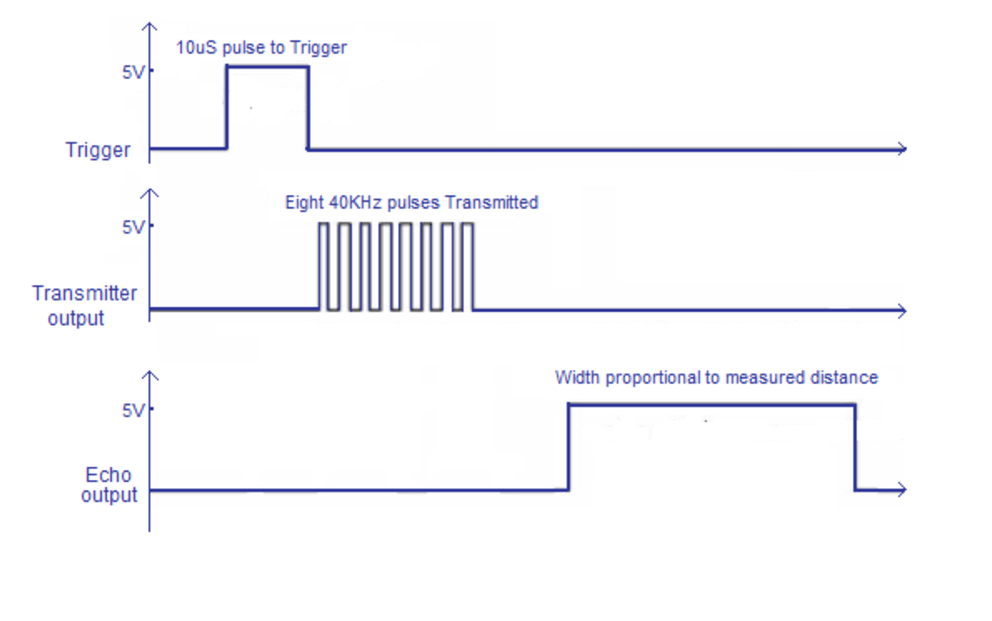
\includegraphics[width=0.7 \textwidth]{HC.eps}
\caption{Diagrama temporal de señales útiles para el sensor HC-SR04.}
\label{HC}
\end{figure}


\begin{enumerate}[(a)]
	\item Busque en Internet información sobre el sensor, como cuántos pines tiene, cómo se usan y cómo configurar los respectivos pines en el Arduino.
	\item Realice un programa en Arduino para medir la distancia que hay entre el sensor y un objeto. Puede enviar el dato a la PC a través del puerto serie y visualizarlo en el monitor serie de Arduino.
	\item Este sensor tiene un cierto rango donde funciona correctamente. Determínelo, realizando mediciones.
	\item El precio de este sensor ronda los $4 $ USD. ¿Le parece que es el sensor más conveniente para esta aplicación? 

\textbf{Nota:} Para utilizar de manera sencilla el sensor, puede resultarle piola la librería \textbf{Ultrasonic.h} que se puede encontrar en la Web. 

\end{enumerate}

\subsubsection*{2 - Usando emisor y receptor infrarrojo}

Puede utilizarse un esquema similar al de los sensores CNY70 para detectar proximidad. Es decir, midiendo reflexión de un rayo irradiado por un emisor infrarrojo con un fototransistor. 
La ventaja de este tipo de sensores es que pueden conseguirse en cualquier local de electrónica, no así con el HC-SR04. Además, tanto el emisor IR como el fototransistor son económicos.

\begin{enumerate}[(a)]
	\item Busque en Internet información y esquemas que utilicen estos componentes al utilizarlos para medir proximidad.
	\item Para regular a qué distancia el receptor detecta al emisor, se debe variar crecientemente la corriente con que se alimenta al emisor. Piense cómo puede armar un ensayo 
	para determinar la relación entre corriente del emisor vs distancia de detección.
	\item El problema que aparece, es que el fototransistor que utilice para recibir el haz reflejado también recibe luz ambiente. Entonces puede que detecte reflexión (en realidad es luz ambiente) sin que el haz 
	infrarrojo haya rebotado en ningún objeto. Lo que se puede hacer para solucionar este aspecto, es alimentar el diodo infrarrojo con una corriente pulsante, de una dada frecuencia. Luego, medir con un pin del Arduino 
	la frecuencia de la señal medida en el fototransistor. Si esta se corresponde con la enviada en el emisor, entonces el haz infrarrojo está rebotando en un objeto. 
	\begin{enumerate}[(i)]
	  \item Busque en la Web ejemplos de aplicación de sensores IR estimulados de dicha manera.
	  \item El método de enviar información ``montada'' en un valor de frecuencia se denomina \textit{modulación}. Investigue sobre \textit{demodulación}, \textit{frecuencia portadora} y \textit{señal moduladora}. 
	  Busque proyectos con microcontroladores donde se utilicen estos términos.
	  \item Investigue sobre el integrado \textit{TSOP1138}. Otro similar es el \textit{IRM2638}. Ambos son demoduladores de frecuencias cercanas a los $38\ kHz$. Los controles remotos convencionales los utilizan. 
	\end{enumerate}

\end{enumerate}


\end{document}
